\subsection{Bottom friction}
%

% - Purpose & Problem description: 
%     These first two parts give reader short details about the test case, 
%     the physical phenomena involved and specify how the numerical solution will be validated
%    
\subsubsection{Purpose}
%

Lorem ipsum dolor sit amet, consectetur adipiscing elit. Vestibulum nec
iaculis mi. Lorem ipsum dolor sit amet, consectetur adipiscing elit. Aliquam
in leo justo. Vestibulum a sem et quam faucibus convallis. Suspendisse id
justo felis, ac venenatis mauris. Aenean enim quam, pellentesque et lobortis
faucibus, faucibus at diam. Quisque interdum dapibus elit ac hendrerit. In
quis metus a neque adipiscing volutpat. Ut a est diam, eget varius lectus.
%
\subsubsection{Description of the problem}
%
Maecenas ipsum nunc, convallis in volutpat ac, sagittis in metus. Pellentesque
habitant morbi tristique senectus et netus et malesuada fames ac turpis
egestas. Quisque a urna dignissim nisl tempus adipiscing ut in libero.
Maecenas auctor semper neque. Nulla facilisi. Phasellus tempus dapibus neque
ac fringilla. Cras euismod adipiscing vulputate. Ut sed aliquam dolor. Aenean
ante dui, porttitor ac venenatis in, condimentum vitae dolor. Nunc velit
ligula, elementum vel gravida eleifend, suscipit eu quam. Donec et est elit.
Vivamus euismod adipiscing mauris, eu convallis mauris suscipit eget. Vivamus
non nibh dolor. Phasellus volutpat consectetur nisl in pretium.
% - Reference: 
%     This part gives the reference solution we are comparing to and 
%     explicits the analytical solution when available;
%    
%
\subsubsection{Reference}
%
Fusce id purus neque, quis vehicula lectus. Pellentesque mi nibh, sagittis id
tincidunt id, condimentum nec quam. Donec orci arcu, sollicitudin auctor
malesuada vitae, pharetra eu justo. Aliquam vel lacus eu libero consequat
dictum. Cras nec dictum dolor. Cras id turpis purus. Vivamus ante orci,
suscipit at auctor ac, tempor id ante. Vivamus sed lectus lectus. Nam tempor
risus vel ipsum aliquam quis mollis turpis posuere.
% - Physical parameters: 
%     This part specifies the geometry, details all the physical parameters 
%     used to describe both porous media (soil model in particularly) and
%     solute characteristics (dispersion/diffusion coefficients, soil <=> pollutant interactions...)
%
%
\subsubsection{Physical parameters}
%
Maecenas ultricies lorem in nisi rhoncus varius. Nullam commodo, purus at
porta tincidunt, sem mauris hendrerit ante, vitae faucibus ipsum urna ut
metus. Donec commodo, nibh nec adipiscing aliquam, metus magna sodales nulla,
a mattis nunc sapien non nisl. Integer eu quam orci. Mauris ut nunc justo,
quis commodo dui. Praesent rutrum, nibh eu laoreet elementum, orci ipsum
auctor lorem, et porttitor tellus ante sit amet mauris. Quisque congue libero
eget urna molestie ullamcorper. Quisque ante augue, dignissim vel cursus eu,
eleifend rutrum nunc. Integer vel velit eros.
% - Geometry and Mesh: 
%     This part describes the mesh used in the computation
%
%
\subsubsection{Geometry and Mesh}
%
Proin auctor elementum posuere. Vestibulum a lorem at felis varius pulvinar in
nec lectus. Aenean in nibh et erat bibendum eleifend et eget odio.
Pellentesque dignissim neque non erat congue at vestibulum lectus convallis.
Curabitur et nisl ut mi fringilla lacinia. Pellentesque ultrices mi non augue
viverra sagittis. Morbi quis lorem nulla, ac viverra nibh. Curabitur
vestibulum diam sit amet mauris rhoncus eu congue lacus adipiscing. Quisque
interdum congue lacus, accumsan placerat nulla varius et. Suspendisse at lacus
non nibh convallis varius quis quis ipsum. Maecenas et quam vitae libero
tincidunt iaculis. In lobortis dictum urna, ac interdum nisi pretium ut. Etiam
sollicitudin fermentum lacus, in tincidunt turpis feugiat in. Proin quis orci
quis diam condimentum ullamcorper.
% - Initial and boundary conditions: 
%     This part details both initial and boundary conditions used to simulate the case 
%
%
\subsubsection{Initial and Boundary Conditions}
%
In hendrerit lobortis libero, eget lacinia erat vestibulum vitae. Nunc vel
ligula ut magna dictum commodo. Nullam mi elit, egestas in bibendum nec,
eleifend a magna. Morbi nunc mauris, suscipit eget fringilla quis, mollis
vitae lorem. Phasellus at eros vel ante iaculis eleifend at vel nibh. Fusce
aliquet metus pretium erat bibendum tincidunt. Ut lorem velit, condimentum eu
volutpat eget, sodales sit amet urna. Nulla sit amet nulla erat. Fusce
bibendum hendrerit eros, quis adipiscing odio adipiscing vel. Donec pulvinar
bibendum nibh quis egestas. Ut vitae erat sed nisl volutpat adipiscing nec ut
libero. Mauris vehicula, mauris sit amet interdum volutpat, est tortor
pellentesque dui, sit amet auctor est mauris non nisl. Aliquam consequat
euismod nisi vel molestie. Nullam est massa, ultrices eu consectetur a,
vulputate quis lorem.
% - Numerical parameters: 
%     This part is used to specify the numerical parameters used
%     (adaptive time step, mass-lumping when necessary...)
%
%
\subsubsection{Numerical parameters}
%
In libero leo, dapibus in iaculis id, faucibus eget diam. Mauris rhoncus nulla
in metus mollis in rutrum tortor eleifend. Quisque facilisis lorem justo, at
lacinia justo. Fusce sapien risus, sagittis vel ornare ac, posuere nec nisl.
Duis condimentum facilisis quam. Donec rutrum mi non est posuere eget sodales
risus adipiscing. Praesent feugiat auctor nisl at consectetur. Curabitur
sollicitudin, augue ac venenatis suscipit, urna metus dapibus lectus, luctus
auctor dolor eros et turpis. Fusce aliquet ullamcorper sem ut fermentum. Ut
purus libero, semper non lobortis vel, suscipit in quam. Nunc vel nisi neque.
Aenean dignissim erat sit amet nulla volutpat vulputate. Integer porta iaculis
magna id elementum. Etiam magna nibh, pharetra ut luctus a, sagittis at ante.
% - Results: 
%     We comment in this part the numerical results against the reference ones,
%     giving understanding keys and making assumptions when necessary.
%
%
\subsubsection{Results}
%
Cras a hendrerit massa. Vestibulum id congue metus. Pellentesque vehicula,
diam quis adipiscing fringilla, libero ipsum laoreet ipsum, ac egestas odio
urna vitae nisi. Sed ac erat at metus cursus luctus quis id nunc. In congue
mauris at tellus euismod sit amet ornare diam rutrum. Fusce malesuada orci a
libero iaculis sit amet porta erat tincidunt. Vestibulum vel ipsum vitae sem
ornare tristique pretium eu erat. Maecenas velit ligula, convallis cursus
adipiscing vel, commodo vel risus.
% Here is an example of how to include the graph generated by validateTELEMAC.py
% They should be in test_case/doc/ or in a subfolder
%\begin{figure} [!h]
%\centering
%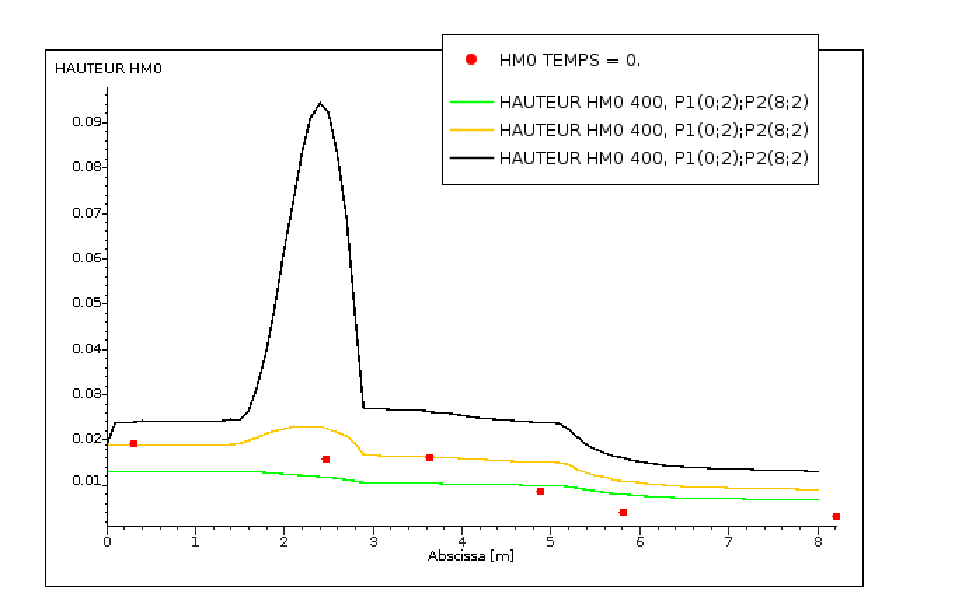
\includegraphics[scale=0.3]{hauteur.png}
% \caption{mycaption}\label{mylabel}
%\end{figure}


